\scanpage{156}
\figure{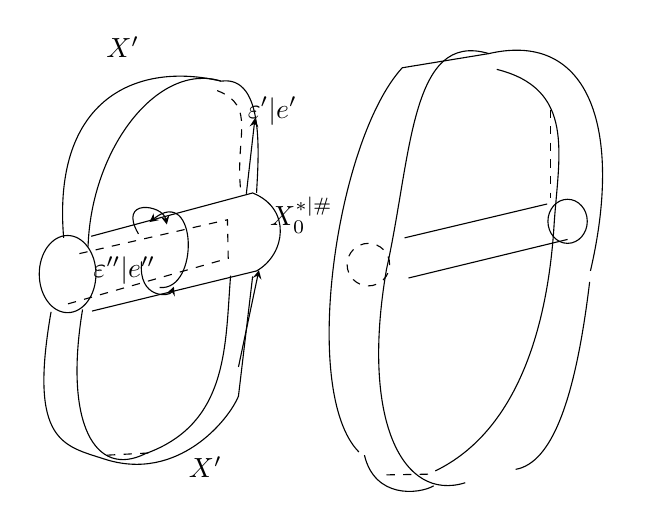
\begin{tikzpicture}[x=1cm,y=1cm,>=stealth]
\draw (-2.65,0) ellipse (.36 and .49);
\draw (-2.7,.46) .. controls (-2.85,2.25) and (-1.75,2.7) .. (-.7,2.45) .. controls (-.13,2.53) and (-.23,1.45) .. (-.25,1.03);
\draw (-2.39,.35) .. controls (-2.35,1.6) and (-1.5,2.7) .. (-.7,2.45);
\draw (-2.86,-.48) .. controls (-3.15,-2.14) and (-2.7,-2.18) .. (-2.18,-2.35) .. controls (-1.25,-2.65) and (-.6,-1.85) .. (-.48,-1.55) -- (-.3,-.03);
\draw (-2.46,-.45) .. controls (-2.7,-1.9) and (-2.3,-2.6) .. (-1.66,-2.28) .. controls (-.6,-1.9) and (-.65,-.9) .. (-.58,-.02);
\draw (-2.35,.48) -- (-.3,1.03) .. controls (.2,.83) and (.12,.25) .. (-.25,.04) -- (-2.34,-.47);
\draw[dashed] (-2.5,.26) -- (-.62,.69) -- (-.61,.2) -- (-2.65,-.38);
\draw[->] (-1.48,-.17) .. controls (-.97,-.22) and (-1,1.14) .. (-1.61,.66);
\draw[->] (-1.75,.51) .. controls (-2.02,.97) and (-1.44,.88) .. (-1.39,.63);
\draw[->] (-1.71,.16) .. controls (-1.76,-.32) and (-1.35,-.29) .. (-1.3,-.16);
\draw[->] (-.48,-1.18) -- (-.22,.05);
\draw[->] (-.38,1.02) -- (-.27,1.98);
\draw[dashed] (-.75,2.33) .. controls (-.24,2.13) and (-.53,1.75) .. (-.45,1.05);
\draw[dashed] (-2.15,-2.3) -- (-1.58,-2.27);
\node at (-1.95,2.88) {$X'$}; \node at (-.9,-2.45) {$X'$};
\node at (.32,.75) {$X_0^{\unsure{*|\#}}$};
\node at (-.05,2.07) {$\unsure{\varepsilon'|e'}$}; \node at (-1.93,.05) {$\unsure{\varepsilon''|e''}$};
\draw (1.05,-2.26) .. controls (.3,-1.5) and (.76,1.7) .. (1.6,2.62) -- (2.7,2.8) .. controls (4,3.1) and (4.4,1.8) .. (3.99,.04);
\draw (2.7,2.8) .. controls (1.7,3.1) and (1.72,1.5) .. (1.4,.06) .. controls (1.07,-1.85) and (1.6,-2.9) .. (2.4,-2.65);
\draw (1.12,-2.3) .. controls (1.25,-2.85) and (1.8,-2.8) .. (2,-2.69);
\draw (2.8,2.6) .. controls (3.8,2.35) and (3.59,1.53) .. (3.53,.65) .. controls (3.45,-.7) and (3.05,-2) .. (2.02,-2.5);
\draw (3.98,-.1) .. controls (3.8,-1.6) and (3.5,-2.4) .. (3.04,-2.48);
\draw (1.63,.46) -- (3.44,.89); \draw (1.68,-.05) -- (3.7,.44);
\draw (3.7,.67) ellipse (.25 and .28);
\draw[dashed] (1.17,.12) ellipse (.27 and .27);
\draw[dashed] (1.4,-2.55) -- (2.01,-2.54);
\draw[dashed] (3.48,2.09) -- (3.48,.97);
\end{tikzpicture}}

\[
\begin{array}{lll}
\tau' & \tau'' & \tau^{\deleted{\unsure{'''}}}\\
\unsure{\varepsilon'|\rho'} & \varepsilon^{\deleted{\unsure{''}}} & \overline\varepsilon'
\end{array}
\]

\figure{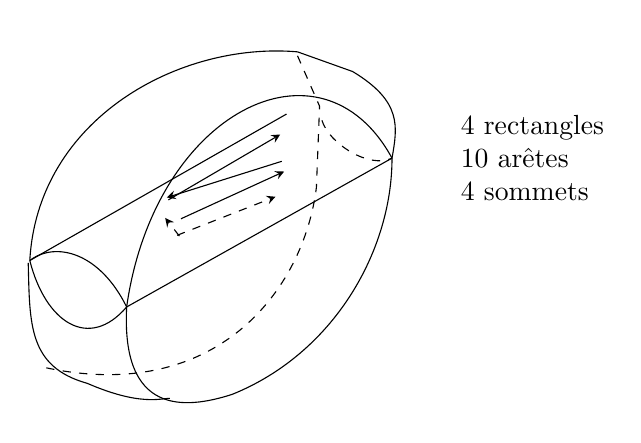
\begin{tikzpicture}[x=1cm,y=1cm,>=stealth]
\draw (-2.3,-.55) .. controls (-2.2,1.25) and (-.4,2.23) .. (1.1,2.1) -- (1.8,1.85) .. controls (2.43,1.47) and (2.37,1.15) .. (2.3,.75);
\draw (-2.32,-.58) .. controls (-2.3,-1.36) and (-2.32,-1.9) .. (-1.57,-2.11) .. controls (-.9,-2.4) and (-.64,-2.3) .. (-.52,-2.3);
\draw (-1.07,-1.14) .. controls (-1.14,-2.5) and (-.35,-2.45) .. (.27,-2.25) .. controls (1.56,-1.73) and (2.3,-.43) .. (2.3,.75);
\draw (-1.07,-1.14) .. controls (-.72,1.34) and (1.4,2.4) .. (2.3,.75);
\draw (-2.3,-.55) .. controls (-1.97,-.3) and (-1.41,-.45) .. (-1.07,-1.14) .. controls (-1.55,-1.7) and (-2.1,-1.34) .. (-2.3,-.55);
\draw (-2.3,-.55) -- (.96,1.31); \draw (-1.07,-1.14) -- (2.3,.75);
\draw[dashed] (1.1,2.05) -- (1.38,1.41) -- (1.34,.38) .. controls (1.18,-.92) and (.07,-2.4) .. (-2.15,-1.9);
\draw[dashed] (1.41,1.23) .. controls (1.5,.93) and (2.02,.61) .. (2.3,.75);
\draw[->] (-.54,.22) -- (.88,1.05); \draw[->] (.9,.71) -- (-.56,.25);
\draw[->] (-.38,-.02) -- (.93,.58); \draw[->,dashed] (-.43,-.23) -- (.82,.26);
\draw[->,dashed] (-.4,-.24) -- (-.58,-.01);
\node[anchor=west,align=left] at (3.05,.75) {4 rectangles\\10 arêtes\\4 sommets};
\end{tikzpicture}}

\figure{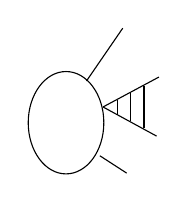
\begin{tikzpicture}[x=1cm,y=1cm]
\draw (0,0) ellipse (.48 and .65);
\draw (.26,.53)--(.72,1.2); \draw (.43,-.42)--(.77,-.64);
\draw (.47,.2)--(1.18,.58); \draw (.47,.2)--(1.15,-.17);
\draw (.65,.1)--(.65,.29); \draw (.82,.02)--(.82,.38); \draw (.99,-.07)--(.99,.47);
\end{tikzpicture}}
\[
\tau^{\prime2}=\tau^{\prime\prime2}=\tau^2
=\deleted{\unsure{(\tau''\tau)^2=\tau\tau''=\tau''\tau'}};
(\tau''\tau)^2=(\tau\tau')^2=(\tau'\tau'')^2=1
\]
\[
\begin{aligned}
\tau(\varepsilon_0)&=\varepsilon_2\qquad(\tau(\varepsilon_2)=\unsure{\tau(\varepsilon_1)|\tau(\varepsilon_0)} )\\
\tau(\varepsilon_1)&=\varepsilon_1^{-1}\\
\tau'(\varepsilon_0)&=\tau''(\varepsilon_0)=\varepsilon_0^{-1}\\
\bigl(\Rightarrow\quad\tau'(\varepsilon_{\unsure{1|2}})&=\tau''(\varepsilon_2)=\varepsilon_2^{-1}\bigr)\\
\tau'(\varepsilon_1)&=\tau''(\varepsilon_1)=\varepsilon_1^{-1}\\
[\varepsilon_0,\varepsilon_2]&=1
\end{aligned}
\]
\margin{$\begin{aligned}
\rho_0&\overset{\mathrm{dfn}}=(\varepsilon_1\varepsilon_0)^{-1}=\varepsilon_0^{-1}\varepsilon_1^{-1}\\
\tau(\rho_0)&=(\varepsilon_1^{-1}\varepsilon_2)^{-1}\overset{\mathrm{dfn}}=\rho_2\\
&=\varepsilon_2^{-1}\varepsilon_1\\
\Rightarrow\quad(\underbrace{\varepsilon_1\varepsilon_0}_{\rho_0^{-1}})^3
&=(\underbrace{\varepsilon_0\varepsilon_1\varepsilon_0}_{\sigma_0})^2
\end{aligned}$}
\figure{\begin{tikzpicture}[x=1cm,y=1cm,>=stealth]
\draw (-3.9,1.9)--(1.1,2.05) .. controls (2.05,2.45) and (2.55,3.6) .. (3.05,4.15);
\node (A) at (-2.6,.88) {$\begin{gathered}(\varepsilon_1\varepsilon_0)^6=1\\\Vert\\(\varepsilon_0\varepsilon_1\varepsilon_0)^4\end{gathered}$};
\draw (-2.62,.88) ellipse (1.55 and 1.05);
\node at (1.1,1.15) {$\varepsilon_0\underbrace{\varepsilon_1\varepsilon_0}_{\rho_0^{-1}}=\underbrace{\varepsilon_1\varepsilon_0}_{\rho_0^{-1}}\varepsilon_1$};
\node (B) at (1.1,-1.15) {$\varepsilon_2\varepsilon_1^{-1}\varepsilon_2=\varepsilon_1^{-1}\varepsilon_2\varepsilon_1^{-1}$};
\draw[->] (-1.11,.35) .. controls (-1.32,-.62) and (-.15,-.59) .. (.1,-.75);
\end{tikzpicture}}

\margin{156}
